\documentclass[10pt]{article}
\usepackage{icmlko}

\icmlmeta{IP 파운데이션 월드모델}{163}{큰 손잡이가 옳은 손잡이다}{무엇이 칸을 크게 만드는지 찾았더니 도메인이 아니라 축이었고, 크기와 정확도의 순위상관이 $+$0.90이었다 --- 여덟 노트짜리 물음이 두 줄로 정리된다}

\begin{document}

\twocolumn[
\icmlheader

\begin{abstract}
노트 162가 ``큰 칸과 작은 칸이 다른 이야기를 한다 --- 무엇이 칸을 크게
만드나''를 남겼다. 후보 다섯을 댔다: 유보 표본 수 · 축의 표준편차 · 축
덮음 · $|$라벨 상관$|$ · 서로 다른 값의 수. \textbf{다섯 다 약하다}
($|\rho| \le 0.33$). 대신 구성을 보니 답이 있었다. \textbf{큰 칸 열여덟에
도메인은 아홉이 고르게 섞여 있는데(각 1$\sim$3) 축은 갈린다} --- 굿즈 규모
7 · 타깃 폭 5 대 장소 노출 1. 작은 칸은 정확히 반대다 --- 장소 노출 6 ·
입장 마찰 6 대 굿즈 규모 1. \textbf{칸 크기는 축의 성질이지 도메인의
성질이 아니다.} 그래서 축별로 다섯 정식화를 다 합쳐 재니 관계가 드러난다.
\textbf{축의 평균 $|$효과$|$ 와 사전 부호 정확도의 순위상관이 $+$0.900이다.}
타깃 폭은 효과 0.059에 \textbf{45/45 = 100\%}, 굿즈 규모는 0.045에
\textbf{39/40 = 98\%}. 반대쪽은 입장 마찰 0.023에 27/40 = 68\%, 장소 노출
\textbf{0.010}에 26/35 = 74\%다. 두 무리로 묶으면 \textbf{큰 축(굿즈 ·
타깃)은 평균 0.052에 부호 99\%(84/85), 작은 축(장소 · 마찰)은 0.016에
71\%(53/75)}다. \textbf{크게 움직이는 손잡이가 옳은 방향으로 움직인다.}
이것이 노트 155부터 여덟 노트를 정리한다. 그동안 ``어느 \emph{정식화}가
손잡이 모형인가''를 물었는데 --- 다섯이 전부 같은 답을 낸다.
\textbf{물음은 정식화가 아니라 축이었다.} 그리고 노트 162의 ``60칸이
필요하다''는 사실상 도달 불가다: 도메인을 늘리면 칸이 다섯 축에 고루
붙으므로 큰 칸은 5분의 2만 는다 --- 18에서 60까지 가려면 도메인이
스물한 개 더 필요하다. \textbf{손잡이 충실도로 정식화 순위를 매기는 길은
닫혔다.} 대신 열린 것이 제품 쪽 문장 하나다 --- \textbf{기획자에게 굿즈
규모와 타깃 폭은 조언할 수 있고 장소와 입장 방식은 조언할 수 없다.}
\end{abstract}
]

\begin{figure*}[t]
\centering
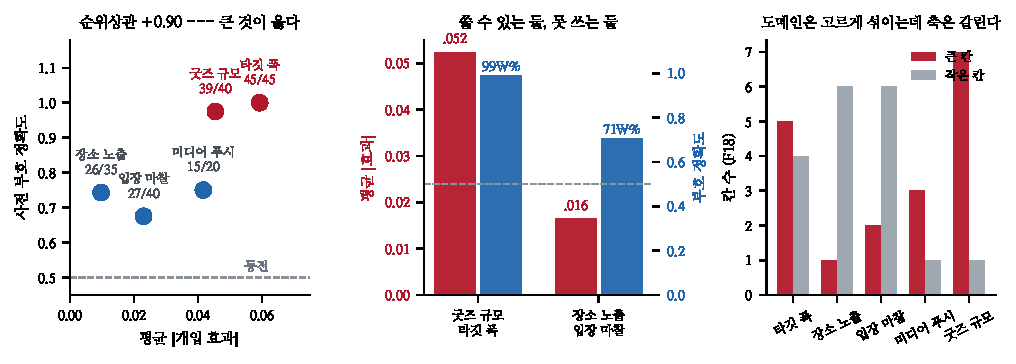
\includegraphics[width=\textwidth]{figs/loud.pdf}
\caption{왼쪽 --- 크기와 정확도의 순위상관 $+$0.90. 가운데 --- 쓸 수 있는
둘, 못 쓰는 둘. 오른쪽 --- 도메인은 고르게 섞이는데 축은 갈린다.}
\end{figure*}

\section{도메인이 아니라 축이다}

\begin{table}[t]
\centering\tsize
\caption{칸 크기($|$효과$|$)를 설명할 후보. 36칸.}
\begin{tabular}{lrr}
\toprule
& F18 & F6 \\
\midrule
서로 다른 값 수 & $+$.220 & $+$.297 \\
축 덮음 & $+$.160 & $+$.044 \\
$|$라벨 상관$|$ & $-$.095 & $-$.068 \\
유보 표본 수 & $-$.123 & $+$.072 \\
축의 표준편차 & $-$.190 & $-$.325 \\
\bottomrule
\end{tabular}
\end{table}

\claimx{\textbf{다섯 다 약하다.} 제일 센 것이 0.33이다. 한 변수로는 칸
크기를 설명 못 한다.}{다섯 다 \emph{연속} 변수로 놓고 잰 것이다. 범주로
보면 다른 그림이 나올 수 있고, 실제로 나왔다.}

\begin{table}[t]
\centering\tsize
\caption{큰 칸 18개와 작은 칸 18개의 구성. F18.}
\begin{tabular}{lrr}
\toprule
& 큰 칸 & 작은 칸 \\
\midrule
\textbf{굿즈 규모} & \textbf{7} & 1 \\
\textbf{타깃 폭} & \textbf{5} & 4 \\
미디어 푸시 & 3 & 1 \\
\textbf{입장 마찰} & 2 & \textbf{6} \\
\textbf{장소 노출} & 1 & \textbf{6} \\
\midrule
도메인 (아홉) & 1$\sim$3씩 & 1$\sim$3씩 \\
\bottomrule
\end{tabular}
\end{table}

\claimx{\textbf{도메인은 고르게 섞이고 축은 갈린다.} 아홉 도메인이 큰
칸에도 작은 칸에도 1$\sim$3개씩 들어 있는데, 축은 굿즈 규모가 7 대 1,
장소 노출이 1 대 6이다. \textbf{칸 크기는 축의 성질이다.}}{축마다 칸이
7$\sim$9개뿐이라 이 분할 자체의 표본이 작다. 다만 굿즈 7:1 과 장소 1:6 은
방향이 뚜렷하다.}

\section{큰 축이 옳은 축이다}

\begin{table}[t]
\centering\tsize
\caption{축별. 정식화 다섯을 다 합쳐 셌다.}
\begin{tabular}{lrrr}
\toprule
& 칸 & 평균 $|$효과$|$ & 부호 정확 \\
\midrule
\textbf{타깃 폭} & 9 & \textbf{.0593} & \textbf{45/45 = 100\%} \\
\textbf{굿즈 규모} & 8 & \textbf{.0454} & \textbf{39/40 = 98\%} \\
미디어 푸시 & 4 & .0417 & 15/20 = 75\% \\
입장 마찰 & 8 & .0230 & 27/40 = 68\% \\
\textbf{장소 노출} & 7 & \textbf{.0097} & 26/35 = 74\% \\
\bottomrule
\end{tabular}
\end{table}

\claimx{\textbf{크기와 정확도의 순위상관이 $+$0.900이다.} 크게 움직이는
손잡이가 옳은 방향으로 움직인다. 타깃 폭은 다섯 정식화 $\times$ 아홉
도메인 \textbf{45칸 전부} 맞는다.}{인과의 방향은 둘 다 가능하다 --- 진짜
효과가 큰 축이라 모형이 크고 정확하게 잡는 것일 수도, 신호가 뚜렷해서
모형이 크게 쓰는 것일 수도 있다. 자료로는 안 갈린다.}

\begin{table}[t]
\centering\tsize
\caption{두 무리로.}
\begin{tabular}{lrr}
\toprule
& 평균 $|$효과$|$ & 부호 정확 \\
\midrule
\textbf{큰 축} (굿즈 · 타깃) & \textbf{.0524} & \textbf{84/85 = 99\%} \\
\textbf{작은 축} (장소 · 마찰) & \textbf{.0164} & 53/75 = 71\% \\
\bottomrule
\end{tabular}
\end{table}

\section{여덟 노트를 정리한다}

\claimx{\textbf{물음이 정식화가 아니라 축이었다.} 노트 155부터 162까지
``어느 정식화가 손잡이 모형인가''를 물었는데, 다섯 정식화가 축에 대해
전부 같은 답을 낸다 --- 타깃 폭 100\% · 굿즈 98\% 대 마찰 68\% · 장소
74\%.}{정식화 사이 차이(18/18 대 17/18)는 노트 162가 잰 대로 1 se 안이고,
축 사이 차이(45/45 대 26/35)는 그 몇 배다. \textbf{큰 신호를 놔두고 작은
신호를 여덟 노트 동안 쫓았다.}}

\claimx{\textbf{그리고 노트 162의 60칸은 도달 불가다.} 도메인을 늘리면
칸이 다섯 축에 고루 붙고 큰 칸은 5분의 2만 는다. 18에서 60까지 가려면
도메인이 스물한 개 더 필요하다.}{축을 늘리는 쪽도 막혀 있다 --- 팝업 전용
다섯 축은 팝업에만 있어 5칸이고, 그중 큰 칸이 몇일지도 모른다.
\textbf{손잡이 충실도로 정식화 순위를 매기는 길은 닫혔다.}}

\section{대신 열린 것}

\claimx{\textbf{제품 쪽 문장 하나가 선다.} 기획자에게 \textbf{굿즈 규모와
타깃 폭은 조언할 수 있고}(다섯 정식화 · 아홉 도메인에서 99\% 같은 방향)
\textbf{장소와 입장 방식은 조언할 수 없다}(71\%, 그리고 효과가 3분의 1).}{조언의
\emph{크기}는 여전히 작다 --- 한 등급 올려 순위가 5$\sim$6\% 움직인다.
``어느 쪽으로''는 말할 수 있고 ``얼마나''는 아직 못 한다.}

\begin{table}[t]
\centering\tsize
\caption{남은 것.}
\begin{tabular}{ll}
\toprule
크기 & 한 등급에 5$\sim$6\% --- 의사결정을 바꾸나 \\
장소·마찰 & 71\%인 이유 --- 교란인가 정의인가 \\
\textbf{미디어 푸시} & 칸이 넷뿐이다 --- 덮음을 늘릴 것 \\
\bottomrule
\end{tabular}
\end{table}

마지막 줄이 값싼 다음 걸음이다. 미디어 푸시는 평균 효과가 0.042로 큰 축에
가까운데 칸이 넷뿐이라(다섯 도메인에 덮음이 없다) 정확도 75\%의 표준오차가
크다. \textbf{덮음을 늘리면 큰 축이 셋이 될 수도 있다} --- 노트 108이 이 축을
4,737건 수집해 붙였으니 나머지 도메인도 같은 길이 있다.

\end{document}
